 %%%%%%%%%%%%%%%%%%%%%%%%%%%%%%%%%%%%%%%%%
% Short Sectioned Assignment
% LaTeX Template
% Version 1.0 (5/5/12)
%
% This template has been downloaded from:
% http://www.LaTeXTemplates.com
%
% Original author:
% Frits Wenneker (http://www.howtotex.com)
%
% License:
% CC BY-NC-SA 3.0 (http://creativecommons.org/licenses/by-nc-sa/3.0/)
%
%%%%%%%%%%%%%%%%%%%%%%%%%%%%%%%%%%%%%%%%%

%----------------------------------------------------------------------------------------
%   PACKAGES AND OTHER DOC%%UMENT CONFIGURATIONS
%----------------------------------------------------------------------------------------

\documentclass[paper=a4, fontsize=11pt]{scrartcl} % A4 paper and 11pt font size

%\usepackage[final]{pdfpages}
\usepackage[utf8]{inputenc}
\usepackage[T1]{fontenc} % Use 8-bit encoding that has 256 glyphs
%\usepackage{fourier} % Use the Adobe Utopia font for the document - comment this line to return to the LaTeX default
\usepackage[polish]{babel} % English language/hyphenation
\usepackage{amsmath,amsfonts,amsthm} % Math packages

\usepackage[usenames,dvipsnames]{color} % Required for custom colors
\usepackage{graphicx}
\usepackage{caption}
\usepackage{subcaption}
\usepackage{listings} % Required for insertion of code

\usepackage{lastpage}
\usepackage{tabularx}

%\usepackage{todonotes}

\usepackage{sectsty} % Allows customizing section commands
\allsectionsfont{ \normalfont\scshape} % Make all sections the default font and small caps

\usepackage{fancyhdr} % Custom headers and footers
\pagestyle{fancyplain} % Makes all pages in the document conform to the custom headers and footers
\fancyhead{} % No page header - if you want one, create it in the same way as the footers below
\fancyfoot[L]{} % Empty left footer
\fancyfoot[C]{} % Empty center footer
\fancyfoot[R]{\thepage \, z \pageref{LastPage}} % Page numbering for right footer
\renewcommand{\headrulewidth}{0pt} % Remove header underlines
\renewcommand{\footrulewidth}{0pt} % Remove footer underlines
\setlength{\headheight}{6.6pt} % Customize the height of the header



\numberwithin{equation}{section} % Number equations within sections (i.e. 1.1, 1.2, 2.1, 2.2 instead of 1, 2, 3, 4)
\numberwithin{figure}{section} % Number figures within sections (i.e. 1.1, 1.2, 2.1, 2.2 instead of 1, 2, 3, 4)
\numberwithin{table}{section} % Number tables within sections (i.e. 1.1, 1.2, 2.1, 2.2 instead of 1, 2, 3, 4)

%\setlength\parindent{0pt} % Removes all indentation from paragraphs - comment this line for an assignment with lots of text

%----------------------------------------------------------------------------------------
%   CODE INCLUSION CONFIGURATION
%----------------------------------------------------------------------------------------

\definecolor{MyDarkGreen}{rgb}{0.0,0.4,0.0} % This is the color used for comments
\lstloadlanguages{C++} % Load Cpp syntax for listings, for a list of other languages supported see: ftp://ftp.tex.ac.uk/tex-archive/macros/latex/contrib/listings/listings.pdf
\lstset{language=C++, % UseCpp
        frame=single, % Single frame around code
        basicstyle=\small\ttfamily, % Use small true type font
        keywordstyle=[1]\color{Blue}\bf, % Perl functions bold and blue
        keywordstyle=[2]\color{Purple}, % Perl function arguments purple
        keywordstyle=[3]\color{Blue}\underbar, % Custom functions underlined and blue
        identifierstyle=, % Nothing special about identifiers
        commentstyle=\usefont{T1}{pcr}{m}{sl}\color{MyDarkGreen}\small, % Comments small dark green courier font
        stringstyle=\color{Purple}, % Strings are purple
        showstringspaces=false, % Don't put marks in string spaces
        tabsize=5, % 5 spaces per tab
        %
        % Put standard Perl functions not included in the default language here
        morekeywords={rand},
        %
        % Put Cppl function parameters here
        morekeywords=[2]{on, off, interp},
        %
        % Put user defined functions here
        morekeywords=[3]{test},
        %
        morecomment=[l][\color{Blue}]{...}, % Line continuation (...) like blue comment
        numbers=left, % Line numbers on left
        firstnumber=1, % Line numbers start with line 1
        numberstyle=\tiny\color{Blue}, % Line numbers are blue and small
        stepnumber=5 % Line numbers go in steps of 5
}

% add new command to include cpp code
\newcommand{\cppscript}[2]{
\begin{itemize}
\item[]\lstinputlisting[caption=#2,label=#1]{#1.cpp}
\end{itemize}

}

%----------------------------------------------------------------------------------------
%   TITLE SECTION
%----------------------------------------------------------------------------------------

\newcommand{\horrule}[1]{\rule{\linewidth}{#1}} % Create horizontal rule command with 1 argument of height

\title{
\vspace*{\fill}
\normalfont
\textsc{Projekt Zespołowy}\\ [20pt]
\horrule{1.5pt} \\[0.4cm] % Thin top horizontal rule
\LARGE Baza danych szeregów czasowych implementowana na klastrze obliczeniowym procesorów graficznych
\horrule{1.5pt} \\[0.1cm] % Thick bottom horizontal rule
\normalsize
\textsc{Specyfikacja Funkcjonalna} \\ [20pt]
\vspace*{\fill}
}

\author{Jakub Dutkowski \\ Karol Dzitkowski \\ Tomasz Janiszewski } % Your name

\date{\normalsize\today} % Today's date or a custom date

\begin{document}
\maketitle

\thispagestyle{empty}
\clearpage

\tableofcontents
\listoffigures

\chapter{}

\clearpage

\vspace{4em}


\section{Abstrakt}
Niniejsza dokumentacja przedstawia wstępne założenia dotyczące projektu zespołowego, którego efektem ma być praca inżynierska.
Dokument zawiera opis przypadków użycia oraz wymagania funkcjonalne oraz proponowany podział prac.

\section{Opis programu}
Celem projektu jest stworzenie bazy danych szeregów czasowych efektywnie korzystającej z wydajności oferowanej przez współczesne
procesory graficzne. Dane powinny być przechowywane i przetwarzane w pamięci kart graficznych. Baza danych oprócz przechowywania
danych powinna umożliwiać szybką ich agregację oraz filtrowanie.

\section{Wymagania funkcjonalne}
    \subsection{Zapisywanie danych}
    Baza danych powinna pozwalać na przechowywanie danych (niekoniecznie w trwały sposób) napływających z różnych źródeł
    równolegle.
    \subsection{Agregowanie i filtracja danych}
    Baza danych będzie zwracała dane z zadanych okresów czasu oraz dla wyspecyfikowanych kwalifikatorów (tag, seria).
    Dane zwracane będą jako lista rekordów zawierających tag, serię, czas i wartość lub jako lista wartości zagregowana
    przy pomocy predefiniowanych funkcji.
        \subsubsection{Funkcje agregujące}
        \begin{itemize}
            \item Sumowanie
            \item Średnia
            \item Max
            \item Min
            \item Odchylenie standardowe
            \item Liczba rekordów o wartościach z zadanego przedziału
            \item Wariancja
            \item Całka
            \item Różniczka
            \item Histogram
        \end{itemize}
    \subsection{Działanie w czasie rzeczywistym (on-line)}
    Wszelkie operacje na danych będą wykonywane w czasie rzeczywistym to znaczy nie będzie wykonywana żadna wstępna agregacja
    danych, a wszystkie zadania będą wykonywane na danych aktualnie znajdujących się na GPU. Istnieje więc możliwość że
    część danych nie zostanie uwzględniona w przygotowywaniu odpowiedzi dla użytkownika gdyż jeszcze nie zdążą być zapisane na
    karcie pomimo że zostały przyjęte do systemu.
    \subsection{Komunikacja}
    Baza danych będzie eksponowała interfejs do komunikacji ze źródłem danych oparty na protokole HTTP i formacie JSON
\section{Wymagania niefunkcjonalne}
    \subsection{Skalowalność}
    Program będzie dobrze skalowalny, tj. nie ma konkretnego limitu na ilość węzłów oraz ilości kart graficznych na węźle.
     Jedyną limitacją w tym przypadku może być tylko wydajność serwera głównego
    \subsection{Ilość przechowywanych danych}
    Górnym limitem na ilość danych przechowywanych na jednej karcie GPU będzie około 80\% pojemności pamięci wewnętrznej karty
    \subsection{Wydajność}
    Ponieważ jest to praca ``badawcza'' program będzie w łatwy sposób konfigurowalny i dający możliwość badania uzyskanej
     przepustowości zarówno ze względu na ilość przepływających zadań jak i zapytań
\section{Przypadki użycia}
    Przedstawione poniżej przypadki użycia przedstawiają podstawowy przebieg operacji.
    \begin{enumerate}
        \item Konfiguracja systemu
        \\Użytkownik chcąc zmienić podstawowe ustawienia systemu korzysta z konfiguracyjnego pliku tekstowego w którym
        zmienia żądane wartości
        \item Uruchomienie/Restart systemu
        \\Użytkownik chce uruchomić/zrestartować system korzystając z jednego polecenia na serwerze głównym
        \item Wprowadzenie danych
        \\Użytkownik chce wprowadzić nowe dane do systemu. W tym celu przygotowuje żądanie HTTP i wysyła je do
        głównego serwera
        \item Odczyt i agregacja danych
        \\Użytkownik chce odczytać dane z systemu i zastosować na nich wybraną metodę agregacji. W tym celu przygotowuje
        żądanie HTTP i wysyła je do głównego serwera. W odpowiedzi otrzymuje wynik zadanej operacji

    \end{enumerate}

\section{Wizja systemu}
    \subsection{Komunikacja CPU - GPU}
    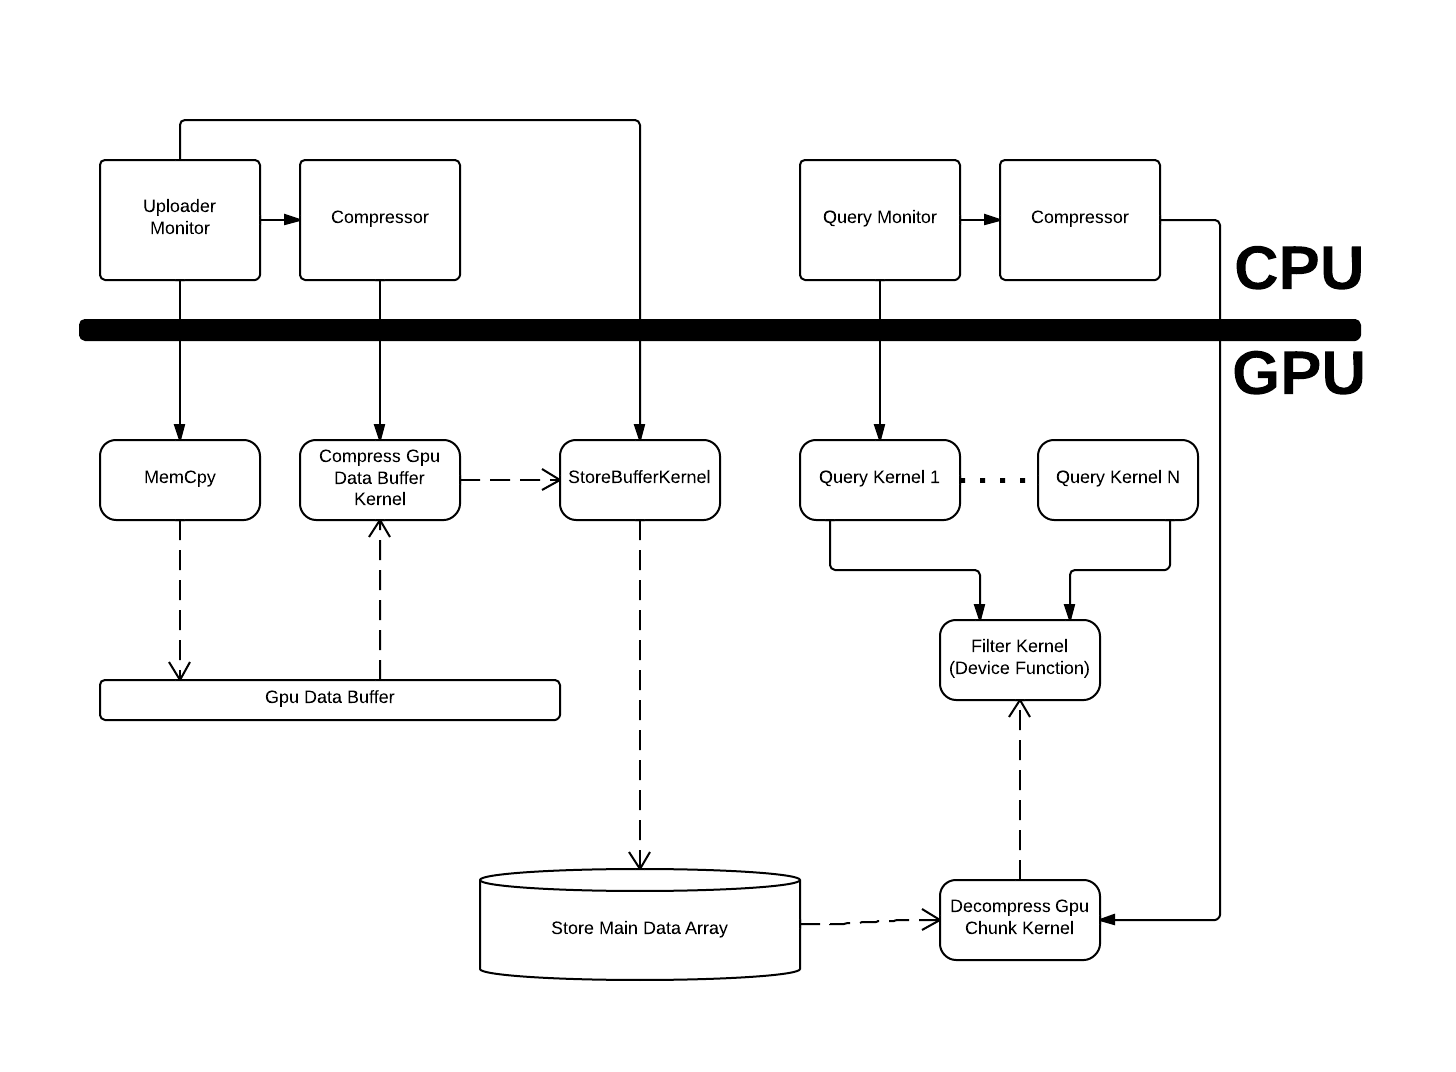
\includegraphics[scale=0.2]{GpuCpu}
    \subsection{Diagram wdrożenia}
    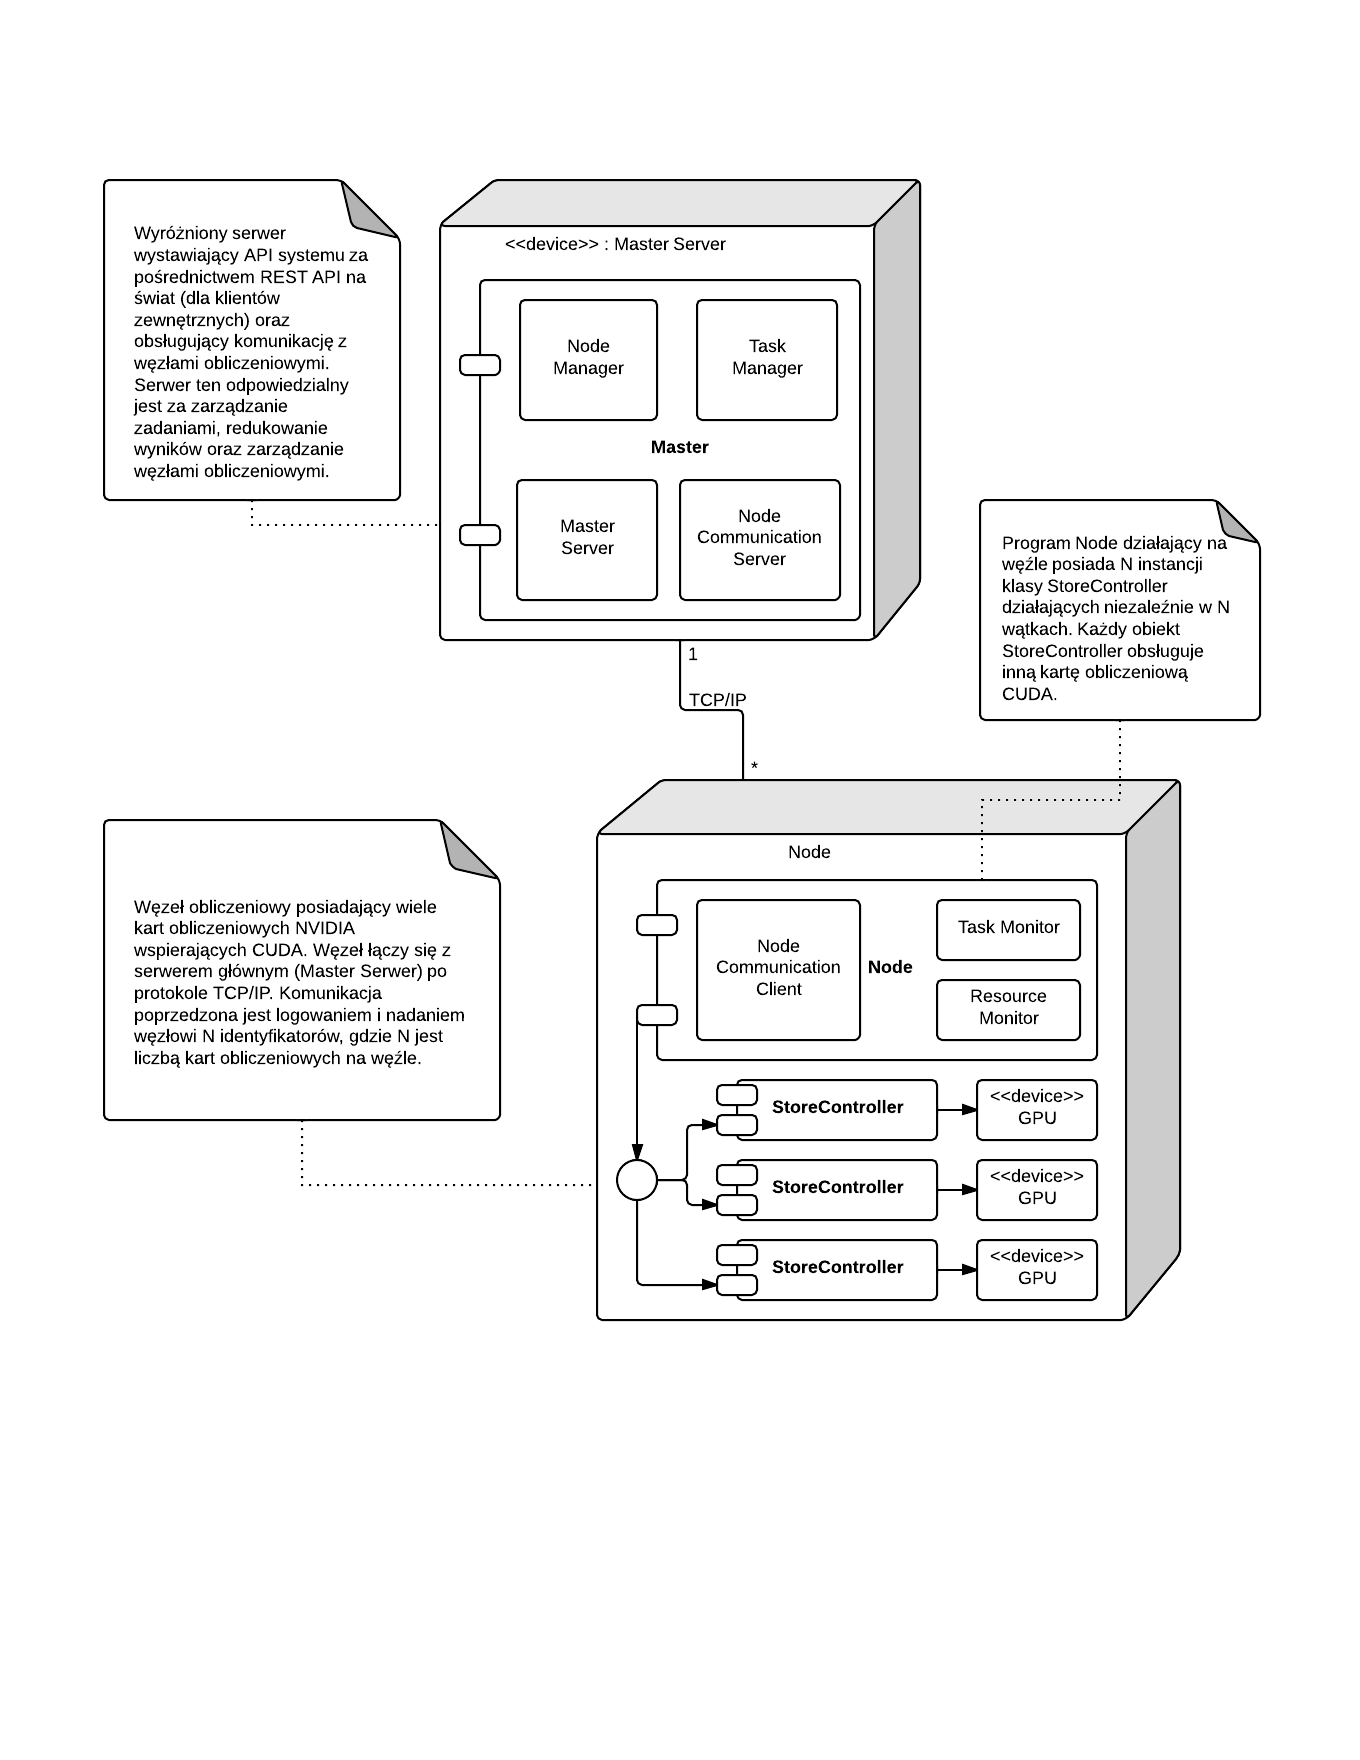
\includegraphics[scale=0.2]{Deployment}

\section{Harmonogram prac}
    \subsection{Metodologia}
    Projekt prowadzony będzie zgodnie z modelem przyrostowym. Na każdym punkcie kontrolnym przedstawiona będzie
    aplikacja rozszerzona o nowe funkcjonalności stanowiące dodatkową wartość dla systemu.

    \subsection{Etapy projektu}
    Wyodrębniono następujące etapy projektu
        \subsubsection{Zapisywanie danych do pamięci karty graficznej}
            System powinien być w stanie przyjąć dane z zewnątrz i zapisać je do pamięci jednej z kart graficznych na jednym z połączonych węzłów.
        \subsubsection{Ekstrakcja danych z bazy danych}
            System powinien móc odpowiedzieć na zadane przez użytkownika zapytania dotyczące przechowywanych danych
        \subsubsection{Poprawa wydajności}
            Na tym etapie cała funkcjonalność powinna być już zaimplementowana. Nastąpi finalna integracja całego systemu
            oraz wdrożenie na wydziałowy klaster obliczeniowy. Dodane zostaną testy integracyjne, zbieranie informacji o stanie węzłów oraz właściwy ``load balancing''. Celem tego etapu będzie eliminacja błędów oraz poprawa wydajności systemu. Poprzez wykonanie testów wydajności powinny zostać przygotowane wskazówki konfiguracji systemu zarówno dla wdrożeń na systemy typu PC jak i serwerowe.
    \subsection{Terminarz}
        \begin{enumerate}
            \item 21-25.10.2013 - Specyfikacja funkcjonalna + stworzenie środowiska pracy, repozytoriów, uzgodnienie technologii i wstępnej architektury systemu
            \item 11-15.11.2013 - Oddanie pierwszego prototypu oraz konkretnej (końcowej) specyfikacji technicznej
            \item 9-13.12.2013 - Oddanie drugiego prototypu oraz testów jednostkowych
            \item 6-10.01.2014 - Oddanie właściwego projektu, testów integracyjnych i wydajnościowych + dokumentacja końcowa
        \end{enumerate}
    \subsection{Podział pracy}
    Przewiduje się poniższy wstępny podział pracy:
        \begin{enumerate}
            \item Jakub Dutkowski
                \begin{itemize}
                    \item kompresja danych na GPU
                    \item komunikacja pomiędzy GPU a CPU
                    \item operacja redukcji dla funkcji agregujących na GPU
                \end{itemize}
            \item Karol Dzitkowski
                \begin{itemize}
                    \item stworzenie struktury systemu dla węzłów rozproszonej bazy danych
                    \item obsługa wprowadzania danych (operacja Insert) dla węzłów
                    \item przetwarzanie/zbieranie i wstępna agregacja danych zwróconych z GPU na węzłach
                    \item oprogramowanie głównej tablicy danych na GPU oraz operacje wstawiania oraz wyjmowania z niej kawałków danych (Chunks'ów)
                    \item obsługa zapytań przychodzących z serwera głównego, zarządzanie zadaniami na węzłach oraz przygotowywanie odpowiedzi dla zadań
                \end{itemize}
            \item Tomasz Janiszewski
                \begin{itemize}
                    \item komunikacja pomiędzy bazą danych a klientem
                    \item komunikacja sieciową pomiędzy elementami systemu
                    \item zarządzanie węzłami po stronie głównego serwera
                    \item przetwarzanie żądań do serwera głównego
                    \item agregacja wyników po stronie serwera głównego
                \end{itemize}
            \item Wspólna praca
                \begin{itemize}
                    \item testowanie
                    \item integracja
                \end{itemize}
        \end{enumerate}

\end{document}